
\section{\textbf{Uncertainty Model}}

\subsection{AR Model Parameter Estimation}

\begin{enumerate}[A)]

\item \textbf{Formulation of the Optimization Problem}

    Denote the number of historical data as $n$ ($n=60$ in our case). We write the auto-regressive model in the matrix form (note that the model depends on the order $p$)
	\[
	\beta_p = \begin{pmatrix} 
		\beta(p+1)  \\
		\beta(p+2)  \\
		\vdots \\
		\beta(n) 
	\end{pmatrix},
	\theta_p = \begin{pmatrix} 
		\theta(1)  \\
		\vdots \\
		\theta(p) 
	\end{pmatrix},
    \epsilon_p = \begin{pmatrix} 
		\epsilon(p+1)  \\
		\epsilon(p+2)  \\
		\vdots \\
		\epsilon(n) 
	\end{pmatrix},
	\]
    \[
    H_p = \begin{pmatrix} 
        \beta(p)   & \beta(p-1) & \cdots & \beta(1)   \\
        \beta(p+1) & \beta(p)   & \cdots & \beta(2)   \\
        \vdots     & \vdots     & \ddots & \vdots     \\
        \beta(n-1) & \beta(n-2) & \cdots & \beta(n-p) \\
    \end{pmatrix}.
    \]
	\[ 
	\beta_p=H_p\theta_p+\sigma_p\epsilon_p, \quad ||\epsilon_p||_\infty \leq 1.
	\]

	Notive that the noice in the autoregressive model is assumed to be genrated based on infinity-norm constraint. Following the noice generation procedure, we estimate the values of $\theta_p$ and $\sigma_p$ by minimizing the infinity norm of the error
	\[
	\min_{\hat{\theta}_p}||\beta_p-\hat{\beta}_p||_\infty, \quad
    \text{s.t. }\hat{\beta}_p = H_p\hat{\theta}_p,
	\]
	This is equivalent to the following LP problem, where we use $\hat{\sigma}$ as an estimate of $\sigma$.
	\begin{equation}\label{eq:ar_opt} 
	\min_{\hat{\theta}_p, \hat{\sigma}_p}\hat{\sigma}_p, \quad
    \text{s.t. }\hat{\beta}_p=H_p\hat{\theta}_p,|\beta_p-\hat{\beta}_p|\preceq\hat{\sigma}_p.
	\end{equation}

\item\textbf{Order Selection for the AR Model}

    The order $p$ of the autoregressive model needs to be determined. Because our goal is to predict the cash flow requirement in the next 6 months, prediction error is important. We use cross-validation on a rolling basis to calculate the prediction error for $1\leq p\leq 30$. The cross-validation procedure is described as follows.\cite{cvTs} For each $p$, 
    \begin{enumerate}
    	\item Fit the model to the data $\beta_1,\cdots,\beta_t$ and let $\hat{\beta}^{(t)}_{t+1},\cdots,\hat{\beta}^{(t)}_{t+6}$ denote the forecasts of the next 6 months. Then compute the error ($e^{(t)}_{t+i} = \beta_{t+i}- \hat{\beta}^{(t)}_{t+i}$) for the forecast observations. 
        \item Repeat step 1 for $t=n-15,\cdots,n-6$ (10-fold). 
        \item Compute : (I) the proportion of absolute error $|e^{(t)}_{t+i}|$ that are greater than the $\sigma$ estimation $|\sigma^{(t)}|$. We call it out-of-bound error.
        (II) MAE (Mean Absolute Error) from the errors $e^{(t)}_{t+i}, t=n-15,\cdots,n-6,i=1,\cdots,6$. 
    \end{enumerate}
    Then, we choose $p$ with the smallest out-of-bound error. For $p$'s with the same out-of-bound error, we choose $p$ with the smallest MAE.

\item\textbf{Results}

     \begin{figure*}
        \centering
        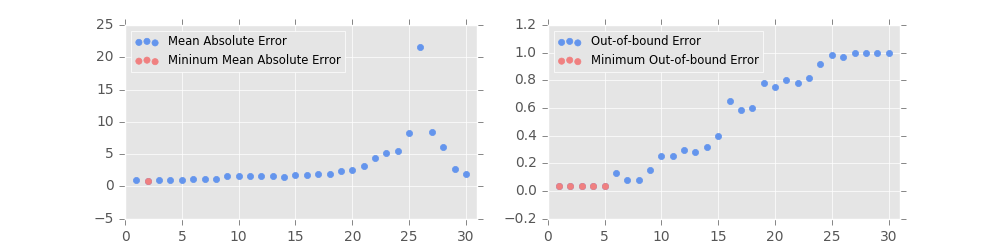
\includegraphics[width=0.7\textwidth]{cv.png}
        \caption{\emph{Cross-validation Results for order selection. Left: The cross-validation MAE for a variety of $p$'s. Right: The cross-validation out-of-bound error for a variety of $p$'s. The minimum error are marked red.}}
        \label{fig:cv_result}
    \end{figure*} 

    \begin{figure*}
        \centering
        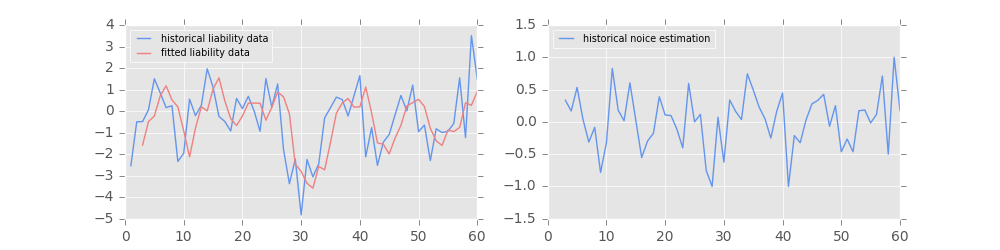
\includegraphics[width=0.7\textwidth]{uncertaintyModel.png}
        \caption{\emph{Visualation of fitted model. Left: The blue line show sthe historical liability data, and the red line shows the fitted value of our model using the order p = 2. Right: The blue line shows the estimation of historical noise $\hat{\sigma}$. Note that the actual prediction error will be multiplied by $\hat{\sigma}$.}}
        \label{fig:uncertaintyModel}
    \end{figure*} 

    The cross-validation results are shown in Figure \ref{fig:cv_result}, the minimum  out-of-bound error and MAE are both attained when $p=2$. We use $p=2$ to solve the optimization problem (\ref{eq:ar_opt}). The corresponding auto-regressive model is given by
    \begin{equation}\label{eq:ar-est}
        \beta(t+1) = \theta_1^*\beta(t) + \theta_2^*\beta(t-1)+\sigma^*\epsilon(t+1),
    \end{equation}
    \[\quad|\epsilon(t+1)|\leq 1.\]
    The solution for the 60 historical data is
    $\sigma^* = 3.243, \theta^*_1 = 0.449, \theta^*_2 = 0.533.$
    Notice that for the rolling-horizon based strategy, the above estimation will only used in January. In future months, the estimation will be updated given new liability data.

\end{enumerate}

\subsection{Uncertainty Model}

    Let $u = (\epsilon(t+1), \cdots, \epsilon(t+T))^T$. With the auto-regressive model (\ref{eq:ar-est}), $\hat{b}(t)$ and $B(t)$ can be expressed as a function of $\beta(t), \beta(t-1), \theta_1^*, \theta_2^*$ and $\sigma^*$ using recursive substitution. The derivation is given in Appendix \ref{apx:recursiveSubstitution}. From the historical data, $\beta(t) = 1.4880$ and $\beta(t-1)=3.5112$. The numerical value is given below
    \[
	   \hat{b}(t) = 
        \begin{pmatrix}
    	2.539 & 1.933 & 2.220 & 2.027 & 2.093 & 2.020
	   \end{pmatrix}^T,
    \]
    \[
	   B(t) = 
        \begin{pmatrix}
    	   3.243 & 0 & 0 & 0 & 0 & 0 \\
            1.456 & 3.243 & 0 & 0 & 0 & 0 \\
            2.382 & 1.456 & 3.243 & 0 & 0 & 0 \\
            1.846 & 2.382 & 1.456 & 3.243 & 0 & 0 \\
            2.098 & 1.846 & 2.382 & 1.456 & 3.243 & 0 \\
            1.925 & 2.098 & 1.846 & 2.382 & 1.456 & 3.243
        \end{pmatrix}.
    \]
    Similar to the AR model parameter, for the rolling-horizon based strategy, the above estimation will only used in January. In future months, the estimation will be updated with the updated AR model.
